\section*{Traceroute}
The traceroute terminal output is shown below in Listing~\ref{list:tracert}. We can see that the traceroute begins first with a hop to the local router at 192.168.2.1, then takes 10 hops to route to 24.156.158.102, with all subsequent hops timing out.

\begin{lstlisting}[caption=Traceroute Terminal Output,label=list:tracert]
tracert compeng4dn4.mooo.com

Tracing route to compeng4dn4.mooo.com [99.236.34.223]
over a maximum of 30 hops:

  1     5 ms     5 ms     5 ms  mynetwork [192.168.2.1]
  2    22 ms    15 ms    19 ms  10.11.2.49
  3     *        *        *     Request timed out.
  4    14 ms    21 ms     *     cksnon1673w_lag37.net.bell.ca [142.124.127.44]
  5     9 ms    18 ms    22 ms  cr01-toroonxnhe9-bundle-ether1.net.bell.ca [142.124.127.159]
  6    22 ms    26 ms    24 ms  bx5-torontoxn_ae0.net.bell.ca [64.230.52.229]
  7    29 ms    28 ms    20 ms  rogers_bx5-torontoxn.net.bell.ca [184.150.158.205]
  8    22 ms    20 ms    21 ms  209.148.235.221
  9    23 ms    13 ms    15 ms  3039-dgw01.hstr.rmgt.net.rogers.com [209.148.237.94]
  10    23 ms    33 ms    18 ms  24.156.158.102
  11     *        *        *     Request timed out.
  12     *        *        *     Request timed out.
  13     *        *        *     Request timed out.
  14     *        *        *     Request timed out.
  15     *        *        *     Request timed out.
  16     *        *        *     Request timed out.
  17     *        *        *     Request timed out.
  18     *        *        *     Request timed out.
  19     *        *        *     Request timed out.
  20     *        *        *     Request timed out.
  21     *        *        *     Request timed out.
  22     *        *        *     Request timed out.
  23     *        *        *     Request timed out.
  24     *        *        *     Request timed out.
  25     *        *        *     Request timed out.
  26     *        *        *     Request timed out.
  27     *        *        *     Request timed out.
  28     *        *        *     Request timed out.
  29     *        *        *     Request timed out.
  30     *        *        *     Request timed out.

Trace complete.
\end{lstlisting}

The WireShark capture was done with a capture filter of \texttt{icmp}. The WireShark capture for traceroute is shown below in Figure~\ref{fig:tracert}. We can see that what the traceroute command does is continually send ICMP echo requests to the targeted hostname (99.236.34.223) from 192.168.2.49 (the \texttt{localhost}). We can also follow the hops in the traceroute by checking the source destination of the "Time-to-live exceeded" ICMP packets, with the first two hops of the traceroute (192.168.2.1 and 10.11.2.49) appearing in the figure.

\begin{figure}[htp]
\centering
\caption[tracert]{Traceroute WireShark Capture}\label{fig:tracert}
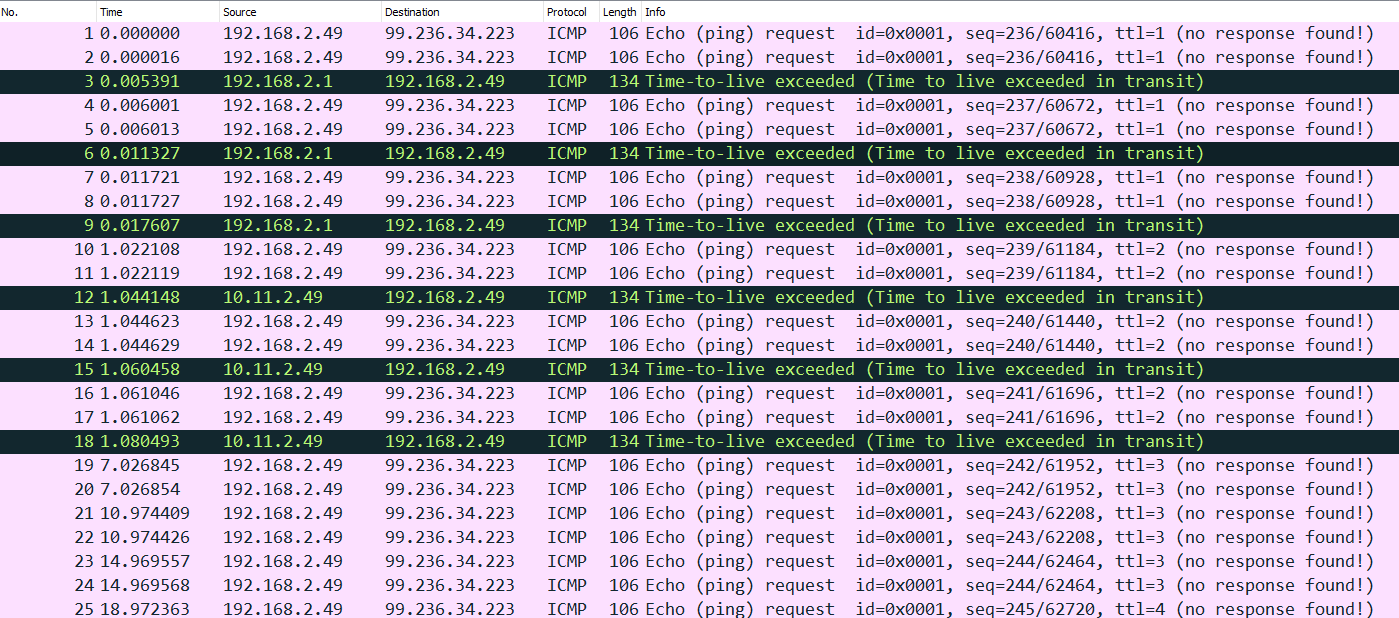
\includegraphics[width=\textwidth]{traceroute_wireshark.png}
\end{figure}